% CLAUDE REPORT::WCD-SPACEFLOOR-0001::2026-11-14T15:00-08:00
% Claude routine "worst-case minimum derivation cost". User follow-up: space lower bound for a 3-SAT algorithm with basic encoding and poly time.
% Role-neutral and additive. It does NOT edit root main.tex or any TMR/LSPV region.
\documentclass[11pt]{article}
\usepackage{amsmath,amssymb,amsthm,graphicx}
\usepackage[margin=1in]{geometry}
\newtheorem{theorem}{Theorem}
\newtheorem{lemma}[theorem]{Lemma}
\title{WCD-SPACEFLOOR-0001: how little space a 3-SAT algorithm can use, given its running time}
\author{Claude scheduled routine (worst-case derivation complexity log)}
\date{2026-11-14 15:00 America/Los\_Angeles}
\begin{document}
\maketitle

\paragraph{Status line.}
\begin{itemize}
\item Theorem~\ref{thm:log} (every 3-SAT machine needs $(1-o(1))\log L$ space, at every time bound): \textbf{PROVED/EXACT}. It is a classical type of argument (Stearns--Hartmanis--Lewis; the equality family is the corpus one from ONETAPE-0001), not a new technique.
\item Theorem~\ref{thm:floor} (floor on space as a function of time exponent): assembled from \textbf{PROVED/EXACT} corpus items and \textbf{KNOWN THEOREMS} cited from memory.
\item Whether a polynomial-time 3-SAT algorithm needs more than $O(\log L)$ space once $c\ge2$: \textbf{OPEN}. A proof of superlogarithmic space for all polynomial-time algorithms would show SAT $\notin$ L; that is open.
\item P versus NP remains \textbf{OPEN}.
\end{itemize}

\section{Encoding and machine}
A formula is written as a header and a list of clauses, each of exactly three literals; a literal is a sign bit and a fixed-width binary variable index. $L$ is the length in bits. The machine has a read-only input and $S$ bits of work memory. Two input models are considered:
\begin{itemize}
\item \emph{sequential}: a two-way input head that moves one cell per step;
\item \emph{random access}: an index tape, counted in $S$, addresses the input.
\end{itemize}

\section{The unconditional floor}
\begin{theorem}\label{thm:log}
Every machine that decides 3-SAT, with any running time, uses space
\[S\ \ge\ \frac{\log_2L-\log_2\log_2L-O(1)}{\log_2 g}\]
on infinitely many lengths in the sequential model ($g$ the work alphabet size, constant depending on the number of states), and $S\ge\log_2L-O(1)$ in the random-access model.
\end{theorem}
\begin{proof}
\emph{Family.} $F_{a,b}=A_a\,P_k\,B_b$ for $a,b\in\{0,1\}^{k}$. $A_a$ forces $x_i=a_i$ with the four-clause gadget on two fresh variables, $B_b$ does the same for $b$, and $P_k$ is a fixed satisfiable padding block. All $F_{a,b}$ with the same $k$ have the same length $L=\Theta(k\log k)$ and the same block boundaries, and $F_{a,b}$ is satisfiable iff $a=b$.

\emph{Sequential model.} Cut the input at the end of $A_a$. A \emph{boundary configuration} is a state, work-tape contents and work-head position, with the input head at the cut; there are $C\le q\,g^{S}(S+1)$ of them. The \emph{table} of a left block records where the machine first crosses the cut from the start, and for each boundary configuration entering the left block, how it next leaves (or that it halts or loops there). There are at most $(C+3)^{C+1}$ tables. The table of the left block and the right block determine the answer. If $A_a$ and $A_{a'}$ with $a\ne a'$ had the same table, then $F_{a,a}$ (satisfiable) and $F_{a',a}$ (unsatisfiable) would get the same answer. So $2^{k}\le(C+3)^{C+1}$, which gives $C\ge\Omega(k/\log k)$ and the stated bound with $\log_2k=\log_2L-O(\log\log L)$.

\emph{Random-access model.} By the skipped-clause argument (WCD-REGIMES-0001, Lemma 2), the machine must read some symbol of every clause of an unsatisfiable $F_{a,b}$, including positions near the end of the input. An index of $S$ bits addresses only $2^{S}$ positions.
\end{proof}
The bound does not use the time. It is weak in absolute terms: for machines with 16 states and a binary work alphabet, the table count forces only $S\ge2,4,9,18$ bits at $k=10^{3},10^{4},10^{6},10^{9}$ (\texttt{spacefloor/raw\_results.json}). It is nevertheless asymptotically the strongest space bound that holds for all polynomial-time algorithms at once.

\section{The floor as time grows}
\begin{theorem}\label{thm:floor}
Let a 3-SAT algorithm run in time $T=L^{c}$.
\begin{itemize}
\item \textbf{Sequential model.} $T\cdot S\ge\Omega(L^{2}/\log L)$ (corpus ONETAPE-0001, crossing sequences over all cuts inside the padding block, on the same family). So $S\ge L^{2-c}/\log L$ for $c<2$.
\item \textbf{Random access.} The checkpoint scheme (WCD-TWOWORLDS-0001) gives $S\ge L^{s(c)}$ with $s(c)=\max_k\frac{k/c^{k-1}-c}{k-1}$, positive for $c<3^{1/3}\approx1.442$. Williams' theorem extends a floor $S\ge L^{\varepsilon}$, $\varepsilon>0$ not explicit, to $c<2\cos(\pi/7)\approx1.80$, infinitely often.
\item \textbf{Every model, every $c$.} Theorem~\ref{thm:log}.
\end{itemize}
\end{theorem}

\begin{center}
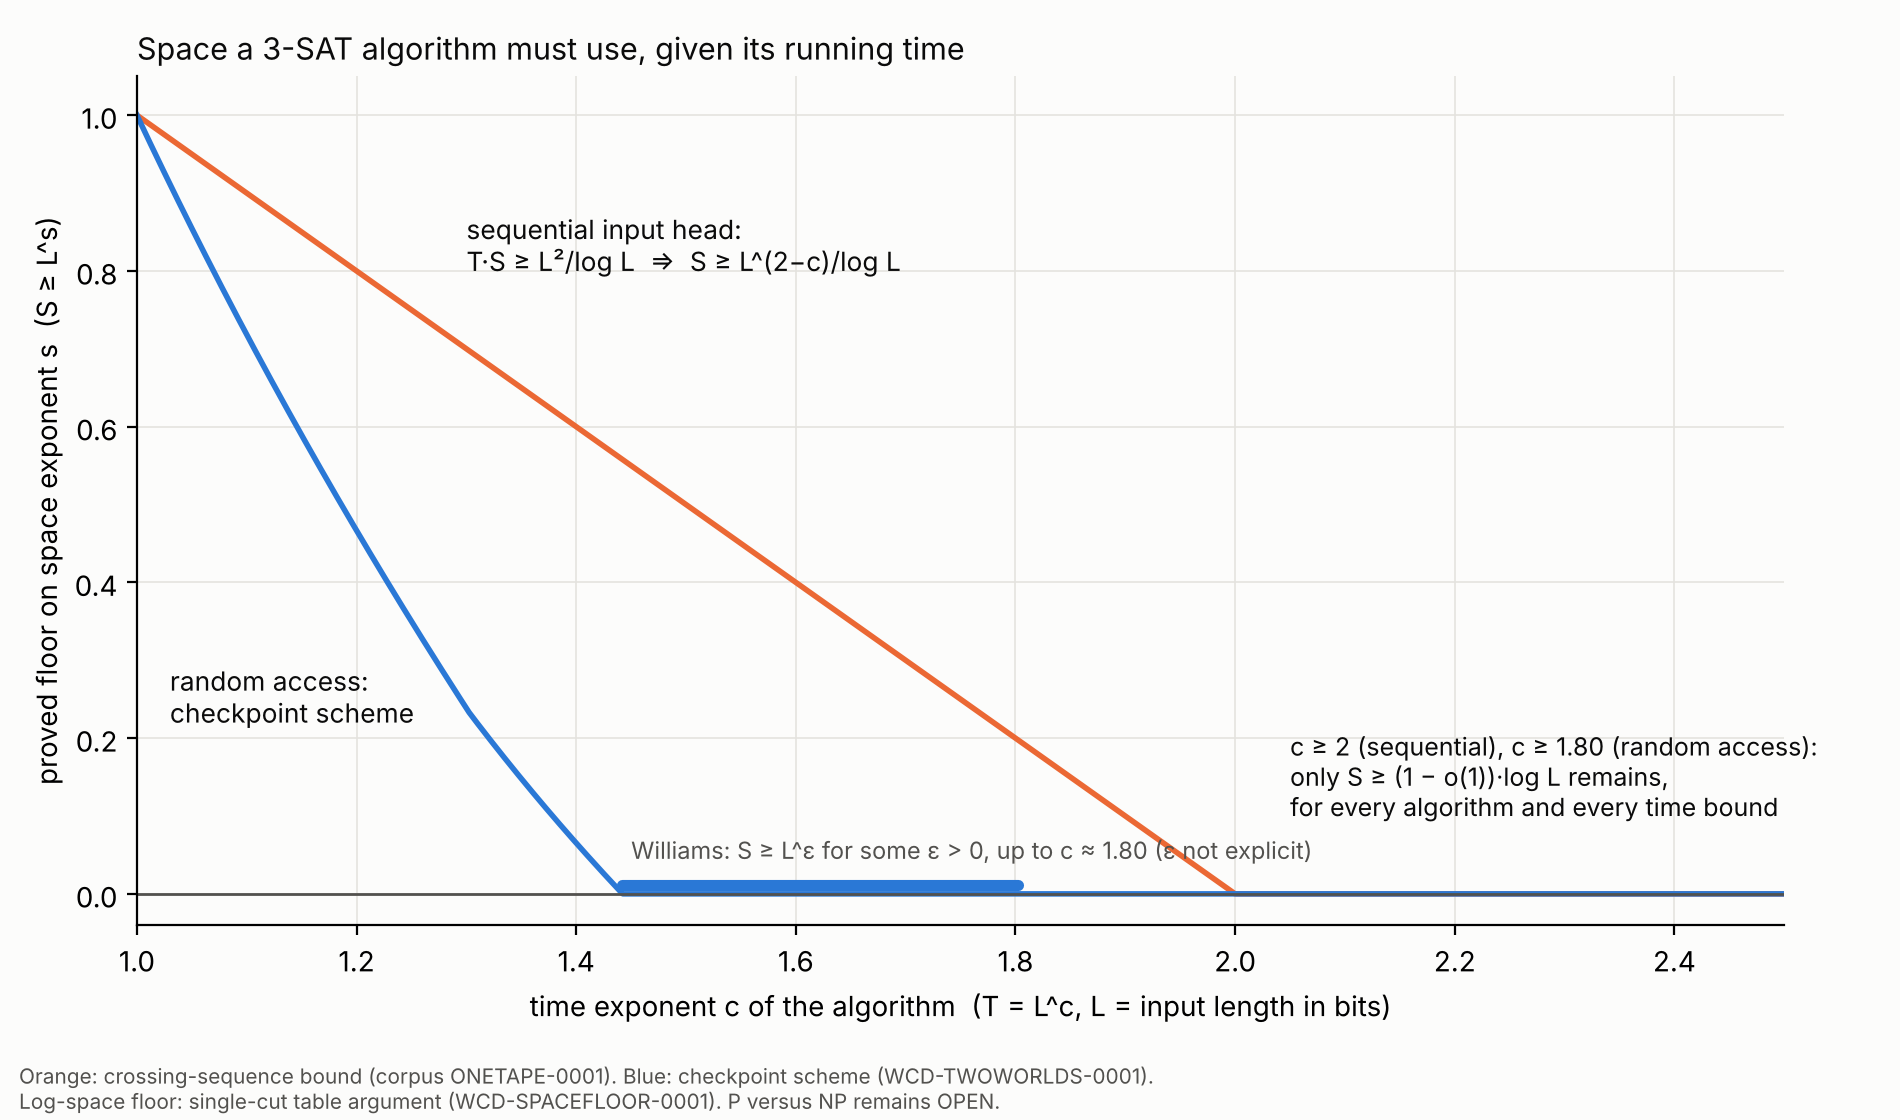
\includegraphics[width=0.95\textwidth]{spacefloor/space_floor.png}
\end{center}

\paragraph{Reading.}
\begin{itemize}
\item As the time exponent rises, the forced space falls: linearly in the sequential model, from $L^{1}$ at $c=1$ to $L^{0}$ at $c=2$; faster for random access, reaching $L^{o(1)}$ at $c\approx1.44$ (this scheme) or $1.80$ (Williams).
\item Beyond those points only the logarithmic floor remains. A polynomial-time algorithm of degree 2 or more is not known to need more than $O(\log L)$ space, and proving it does would separate NP from L.
\item The sequential bound beats the random-access one at every $c$; the extra power of random access is exactly what the corpus barrier L34 isolates.
\end{itemize}

\section{CORPUS REVIEWED / DUPLICATION AUDIT / CHANGES}
\begin{itemize}
\item \textbf{Corpus reviewed:} \texttt{research/agents/claude/onetape/} (README, both source notes, \texttt{verify\_family.py}); the earlier reports of this session; the consolidated living log; world-ledger rows L13, L34, L38--L40 as summarised in AGENTS.md.
\item \textbf{Duplication / contradiction audit:} the sequential $T\cdot S$ tradeoff is ONETAPE-0001, reused, not re-proved. Theorem~\ref{thm:log} uses the same family at a single cut; no corpus entry states the log-space floor. No contradiction found.
\item \textbf{What changed relative to root main:} nothing; \texttt{main.tex} is not edited.
\item \textbf{Adopted:} ONETAPE-0001's family and tradeoff; the checkpoint frontier. \textbf{Rejected / retired:} none.
\item \textbf{Stale or overstated claims found:} none.
\end{itemize}

\section{Evidence}
\texttt{spacefloor/space\_floor.py} re-checks the family exhaustively for $k\le4$ (one length per $k$; satisfiable iff $a=b$ on all $4^{k}$ pairs), computes the table bound for sample machine constants, and draws the figure. Output in \texttt{spacefloor/raw\_results.json} and \texttt{spacefloor/space\_floor.png}; a few seconds. No TeX engine was available, so this file was not compiled.

\medskip\noindent P versus NP remains OPEN. One OPEN load-bearing arrow means P $\ne$ NP is not proved.
\end{document}
% END_OF_VERIFIED_REPORT::CLAUDE::WCD-SPACEFLOOR-0001
